% Hand-in memo: 3 pages plus a 4th for future work. Build with `make memo` (Tectonic).
% Yellow TBD boxes mark numbers that come from #34; remove \draftnote when final.
\documentclass[11pt,a4paper]{article}

\usepackage[margin=1.9cm,top=1.6cm,bottom=1.7cm]{geometry}
\usepackage{lmodern}
\usepackage{microtype}
\usepackage[dvipsnames]{xcolor}
\usepackage{tikz}
\usepackage{graphicx}
\usetikzlibrary{arrows.meta,positioning,fit,backgrounds,calc}
\usepackage{booktabs,tabularx,array}
\usepackage{enumitem}
\usepackage{titlesec}
\usepackage[font=small,labelfont=bf,skip=4pt]{caption}
\usepackage[hidelinks]{hyperref}

\setlist{nosep,leftmargin=1.2em,itemsep=1pt}
\titlespacing*{\section}{0pt}{8pt}{3pt}
\titleformat{\section}{\large\bfseries}{\thesection}{0.6em}{}
\setlength{\parskip}{3pt}
\setlength{\parindent}{0pt}
\renewcommand{\arraystretch}{1.15}

\newcommand{\tbd}[1]{\colorbox{yellow!45}{\scriptsize\sffamily TBD: #1}}
\newcommand{\draftnote}[1]{\par\colorbox{yellow!25}{\parbox{\dimexpr\linewidth-2\fboxsep}{\footnotesize\sffamily Draft: #1}}\par}
\newcommand{\code}[1]{\texttt{\small #1}}

\definecolor{ink}{HTML}{2B2B2B}

\begin{document}

{\raggedright\LARGE\bfseries Agent Copilot: build voice agents like software, watch them at scale\par}
\vspace{2pt}
{\small Prosper challenge, Phase 2 \quad·\quad Feliu Serra Burriel \quad·\quad October 2026}
\draftnote{written before the build, to fix the story and the scope. Numbers come from the final runs.}

\section{The problem}

Prosper's deployment team spends its time on two manual workflows: turning a clinic's guidelines into a working voice agent, and refining agents from issues that clients flag or that show up in calls. We asked Prosper three questions, and the answers set the scope:
\begin{itemize}
  \item Most time goes to turning rules into an agent and checking that it behaves, not to getting the rules from the client.
  \item Agents start from a template per use case and are always customized. Between two small clinics, what changes is mostly tables (appointment types, which provider does which, which insurance covers which visit, the fields needed to register a patient) plus flow and tone.
  \item One person manages fewer than 10 agents, and an agent can take 50,000 calls a month. How to find problems in them is left to us.
\end{itemize}

So there are two bottlenecks. \textbf{The team's:} building an agent and checking it. \textbf{Each agent's:} the places in its graph where calls stall, leak or go wrong. At up to 500,000 calls a month per person nobody can listen, and the scarce resource is attention, not model cost.

\textbf{Thesis.} Coding agents work because code comes with a spec, tests they can run and bug reports with evidence. Voice agents have none of these, which is why both workflows are manual. The Copilot creates them, then works the loop a coding agent works (Figure~\ref{fig:loop}).

\begin{figure}[h]
\centering
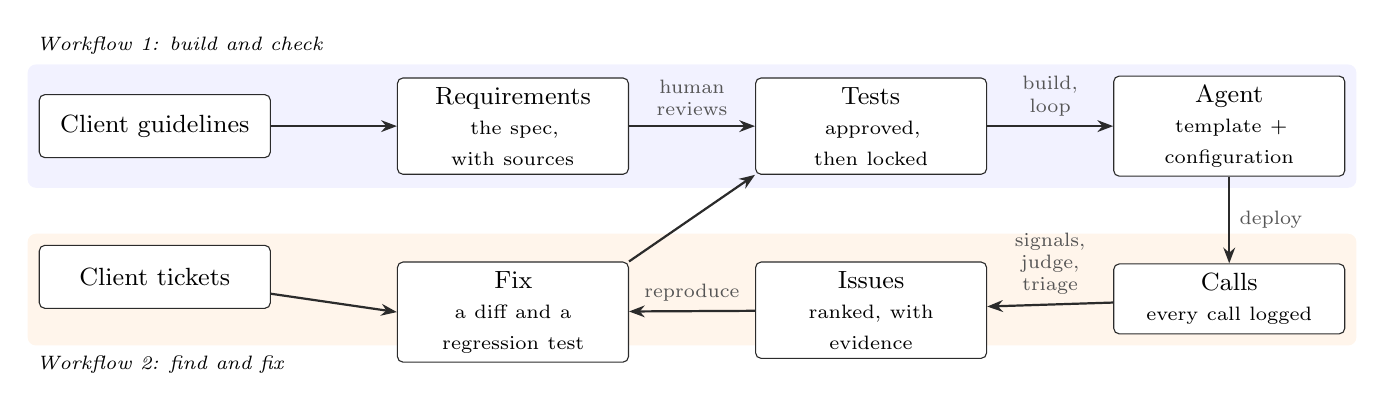
\begin{tikzpicture}[
  box/.style={draw=ink,rounded corners=2pt,align=center,font=\small,minimum height=8mm,text width=27mm,fill=white},
  arr/.style={-{Stealth[length=2mm]},thick,draw=ink},
  lab/.style={font=\scriptsize,align=center,text=ink!80},
  node distance=6mm and 16mm]
  \node[box] (g) {Client guidelines};
  \node[box,right=of g] (r) {Requirements\\\scriptsize the spec, with sources};
  \node[box,right=of r] (t) {Tests\\\scriptsize approved, then locked};
  \node[box,right=of t] (a) {Agent\\\scriptsize template + configuration};
  \node[box,below=11mm of a] (c) {Calls\\\scriptsize every call logged};
  \node[box,below=11mm of t] (i) {Issues\\\scriptsize ranked, with evidence};
  \node[box,below=11mm of r] (f) {Fix\\\scriptsize a diff and a regression test};
  \node[box,below=11mm of g] (k) {Client tickets};
  \draw[arr] (g) -- (r);
  \draw[arr] (r) -- node[above,lab]{human\\reviews} (t);
  \draw[arr] (t) -- node[above,lab]{build,\\loop} (a);
  \draw[arr] (a) -- node[right,lab]{deploy} (c);
  \draw[arr] (c) -- node[above,lab]{signals,\\judge,\\triage} (i);
  \draw[arr] (k) -- (f.west);
  \draw[arr] (i) -- node[above,lab]{reproduce} (f);
  \draw[arr] (f.north east) -- (t.south west);
  \begin{scope}[on background layer]
    \node[fill=blue!5,rounded corners=3pt,inner sep=4pt,fit=(g)(a),label={[font=\scriptsize\itshape,anchor=south west]north west:Workflow 1: build and check}] {};
    \node[fill=orange!8,rounded corners=3pt,inner sep=4pt,fit=(k)(c),label={[font=\scriptsize\itshape,anchor=north west]south west:Workflow 2: find and fix}] {};
  \end{scope}
\end{tikzpicture}
\caption{The loop. A ticket without a call becomes a new or changed requirement.}
\label{fig:loop}
\end{figure}

\section{Workflow 1: from guidelines to a checked agent}

\begin{itemize}
  \item \textbf{Clinic rules are data, not prompts.} Tables and numbers (appointment types, providers per type, coverage, required fields, the cancellation fee) go into a validated clinic configuration that the tools enforce: \code{book\_appointment} refuses a visit the provider does not do, with a reason the model can act on. A new clinic is a configuration plus a small diff on the scheduling template, not a new graph, and the human reviews the configuration as tables.
  \item \textbf{Requirements are the spec.} The Copilot turns guidelines into numbered requirements, each citing the sentence it came from, plus questions for the client where the guidelines are silent, each with the safe default used meanwhile. A healthcare baseline is always added: emergencies, no medical advice, identity before any booking, a human on request.
  \item \textbf{The human reviews tests, not prompts.} Checking 20 one-line tests against the guidelines takes minutes; reading every prompt in a graph takes an hour. Tests are approved before the graph exists and then locked, so the Copilot cannot pass by editing them.
  \item \textbf{Exact checks first, a judge for the rest.} A small model plays a caller with a persona, a goal and facts, through a text runner that follows the voice runtime's rules. What the agent did is checked exactly: tools called, their arguments and order, and how the call ended. A model judge checks what it said: read-backs, privacy, emergencies, medical advice, and that every time and fact came from a tool.
  \item \textbf{Loop, then one diff.} The Copilot edits through validated operations, reruns the failing tests (at most 3 rounds) and proposes one diff to accept or reject like a pull request; while tests fail, the proposal is blocked and says why (the broken link per failure, client questions, tests it doubts). The loop has not paid off yet: \$12.38 against \$2.11 without it, for the same score.
\end{itemize}

\textbf{Why ``all tests pass'' means something.} A model writes the agent, plays the caller and grades the call, so it can agree with itself. Against that: a 20-test reference suite the Copilot never sees; mutation testing (12 of 15 broken agents fail a test; of the 3 that pass, two drop a rule that holds anyway, and one skips the spelling, which a simulated caller can check by reading but a real one cannot); a judge calibrated on hand-labelled calls (below 90\% agreement, a rule becomes an exact check); a check that no test data (names, birth dates) appears in the agent; and a second clinic written by a person and kept out of the repo until the final run.

\section{Workflow 2: finding problems in 500,000 calls a month}

A call through our agents is not a free-form conversation: it is a path through a known graph. Every call already emits its node transitions, so every call is a row in an event log, with no model call at all. Detection starts there, and the graph tells us what kind of failure we are looking at:

\begin{center}\small
\begin{tabularx}{\linewidth}{@{}l X l@{}}
\toprule
\textbf{Shape} & \textbf{What it looks like} & \textbf{Found by} \\
\midrule
Stall & back to the same or an earlier node, or a long visit: a name speech-to-text keeps garbling & transitions \\
Leak & hang-ups in a node where callers should not hang up & transitions \\
Detour & an edge taken more often than it should be, such as needless transfers & transitions \\
Tool error & a tool keeps refusing: a booking field the agent never asks for & tool results \\
Silent failure & the path looks right, the outcome is wrong: the wrong name, an invented slot & judge, clinic records \\
\bottomrule
\end{tabularx}
\end{center}

Three tiers, cheapest first:
\begin{enumerate}[leftmargin=1.4em]
  \item \textbf{Signals on every call, no model.} Per node: entries, exits per edge, turns spent, re-entries, hang-ups, transfers, tool errors. From the clinic system: the same number calling back within 48 hours, a booking cancelled or changed within a day, a new patient record that matches an existing one's birth date and phone under another name. That last one is the ticket ``Mrs.\ Lopez was booked under someone else's name'', found without reading a transcript.
  \item \textbf{A model judge on a sample.} Calls flagged by tier 1, plus a random sample, are checked against the clinic's requirements and a general checklist. Each issue gets a severity, the requirement, the node and quotes. A random sample of 300 calls contains at least one example of any failure that affects 1\% of calls with 95\% probability ($1-0.99^{300}$); for an agent at 50,000 calls a month that is under 3\% of a week's traffic.
  \item \textbf{Triage.} Issues are grouped by node, requirement and shape, and ranked by severity, calls affected and trend. The output is a short list per person, not a dashboard, for example (from the synthetic logs): \emph{Riverside, Confirm name: re-entries at 8.9\% of calls since version 3, against 2.0\% in version 2 and 2.4\% at other clinics, about 680 more calls a week, 3 example calls.}
\end{enumerate}

\begin{figure}[b]
\centering
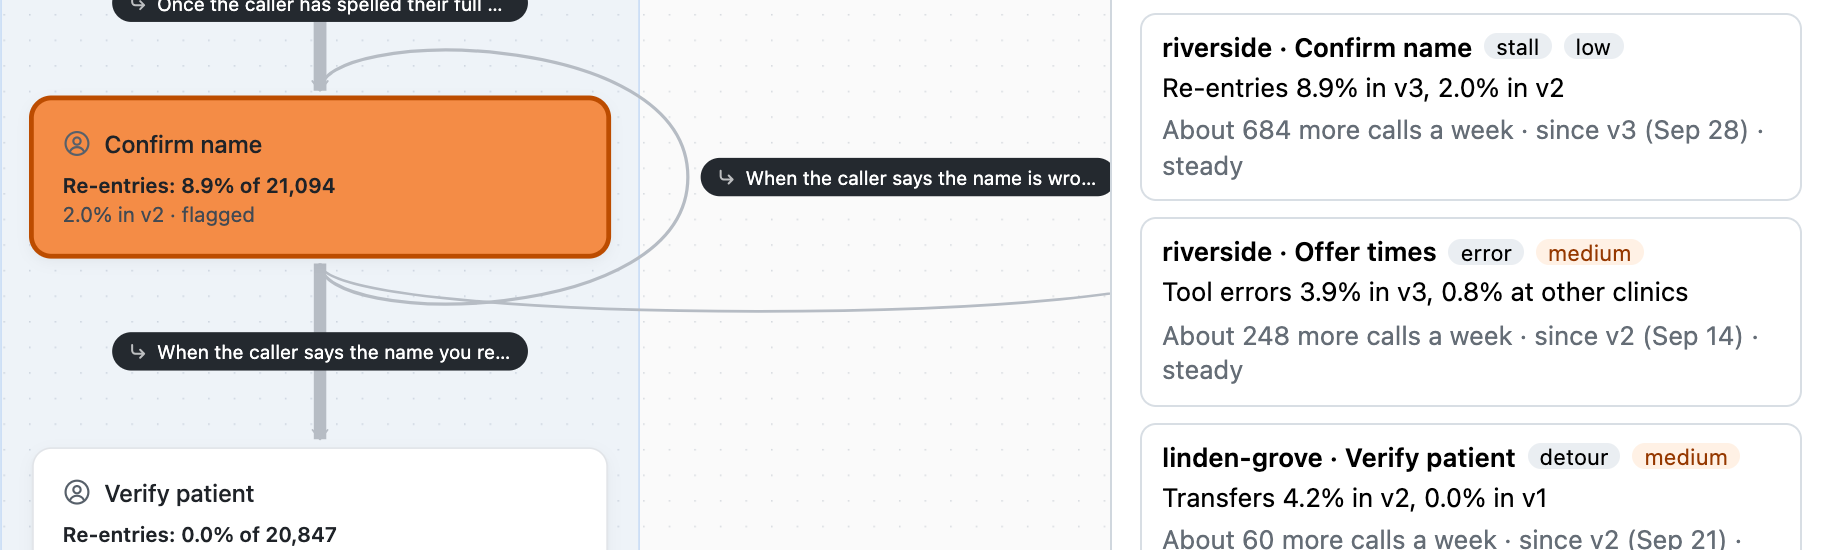
\includegraphics[width=0.72\linewidth]{heatmap.png}
\caption{The call heatmap on the synthetic logs (crop): Riverside, version 3 against 2, re-entries. Confirm name, the planted stall, is the only tinted node (8.9\% against 2.0\%). Edge width is traffic; right, the ranked issues.}
\label{fig:heat}
\end{figure}

\textbf{Baselines make a rate mean something.} Hang-ups after a cancellation are normal. Each node is compared with itself in the previous version, so an accepted change that makes things worse raises an alarm, and with the same template node in other clinics: because agents come from a template, Confirm name at clinic A can be compared with Confirm name everywhere else. Templates give a fleet-wide baseline for free. A two-proportion test with a minimum effect size keeps a busy agent from flagging tiny differences and a quiet one from flagging noise.

\textbf{The heatmap is the view, not the detector.} Opening a ranked issue shows the canvas with nodes tinted by their distance from the baseline, edges drawn by traffic, and collapsed stages rolling up their nodes (Figure~\ref{fig:heat}). From there: the example calls at the quoted turn, then \emph{fix from this issue}: reproduce the call in the text runner from the words speech-to-text heard, find the turn that decided it, fix, and keep the reproduction as a regression test.

\section{Scope: built, mocked, left out}

\begin{center}\small
\begin{tabularx}{\linewidth}{@{}>{\raggedright}p{0.33\linewidth} l X@{}}
\toprule
\textbf{Part} & \textbf{Status} & \textbf{Why} \\
\midrule
Graph editor, test calls with live node highlighting & Built & Phase 1: everything else sits on it. \\
Clinic tools and calendar & Mocked & No access to a real clinic system; tools are where clinic rules are enforced. \\
Text runner and test format & Built & A simulated call costs cents and runs in seconds. \\
Clinic configuration and template & Built & The interviewer's answer 2: clinics differ mostly in tables. \\
Spec, tests, build, loop & Built & Workflow 1, where the team's time goes. Its UI (\#31) is next. \\
Production calls & Mocked & No real call data: 85,000 synthetic call logs from 3 clinics on one template (one at 50,000 calls a month), defects planted at known rates; about 20 simulated calls for silent failures. \\
Signals, triage, heatmap & Built & Workflow 2, the part the brief left open. \\
Judge on a sample & \tbd{planned} & Failures the path cannot show. \\
Fix from an issue: reproduce, fix, regression test & \tbd{planned} & Closes the loop. No forecast of how the call would have gone. \\
Intake call and client checklist & Left out & Getting the rules is not the bottleneck (answer 1). \\
Telephony, rollout and rollback, auth, PHI redaction, other languages & Left out & Production infrastructure, not the Copilot. \\
\bottomrule
\end{tabularx}
\end{center}

\section{Results and limits}

\begin{center}\small
\begin{tabularx}{\linewidth}{@{}X l@{}}
\toprule
\textbf{Measure} & \textbf{Result} \\
\midrule
Reference suite, Copilot-built agent: clinic A, and clinic B held out until the final run & A: 13 of 20 so far; \tbd{\#34} \\
Broken agents caught by the tests; judge agreement with hand labels & 12 of 15; 32 of 32 \\
Planted defects found by signals and triage; false alarms & 6 of 6; none in 18 clinic-weeks \\
Silent failures found by the judge on the 20 simulated calls & \tbd{\#32} \\
Minutes from guidelines to all tests passing, and from issue to accepted fix & \tbd{\#34} \\
Cost per test run and per judged call & \tbd{spend log} \\
\bottomrule
\end{tabularx}
\end{center}

\noindent\begin{minipage}[c]{0.5\linewidth}
\textbf{Where detection stops.} One node's re-entries raised over a 2\% base, at five sizes and three volumes: the share of 10 seeds flagged within two weeks of the version that caused it (10 false alarms in those 600 clinic-weeks).
\end{minipage}\hfill
\begin{minipage}[c]{0.47\linewidth}\footnotesize\setlength{\tabcolsep}{3.5pt}
\begin{tabular}{@{}r ccccc@{}}
\toprule
Calls a week & +0.5 pt & +1 pt & +2 pt & +3 pt & +5 pt \\
\midrule
150 & 0\% & 0\% & 20\% & 50\% & 70\% \\
1,500 & 10\% & 40\% & 100\% & 100\% & 100\% \\
11,500 & 60\% & 100\% & 100\% & 100\% & 100\% \\
\bottomrule
\end{tabular}
\end{minipage}

\smallskip

\textbf{What this does not show.} Text tests do not see latency, interruptions, audio, or speech-to-text errors other than the ones replayed from real calls. Synthetic logs prove the statistics and the plumbing, not how real callers behave; real rates and baselines are learned in production. In production the final judge is real outcomes: completed bookings, callbacks and hang-ups.

\section{Future work: say which tools are missing}

The Copilot does not write tools. Each catalog tool stands for an integration with the clinic's scheduling or records system, and the exact tests only mean the same thing on every agent because all agents share the catalog. The Copilot picks tools from it and fits their parameters to the clinic's configuration. What it should add is a report of the tools it needed and did not have, so the gap reaches a person instead of being papered over in a prompt.
\begin{itemize}
  \item \textbf{At build time, next to the client questions.} The build already lists every requirement it leaves uncarried, each with a free-text reason, but the list mixes ``the template or the tools already do this'' with ``the agent cannot do this''. The second becomes a kind of its own, \emph{needs a tool}: it names the missing capability (``text the patient a confirmation'', ``put the caller on a waitlist''), cites the guideline sentence and states what the agent does in the meantime: says it cannot, takes a message, or transfers. The reviewer sees it next to the questions for the client.
  \item \textbf{In production, on the heatmap.} The judge on a sample (tier 2) tags calls where the caller asked for something the agent had no tool for, along with the transfer or hang-up that followed. Triage counts these by node and by request across the fleet, which is meaningful because every clinic runs the same template: for example, a waitlist asked for at Find slots at every clinic, with its share of calls and example calls. The heatmap gains one more layer: where callers ask for what the agent cannot do.
  \item \textbf{The output is a ranked integration backlog.} Each entry lists the requirements that need it, the clinics that asked, the calls it would have changed, and quotes. Adding a tool stays a person's decision and an engineer's job. The Copilot shows which one is worth building next.
\end{itemize}

\end{document}
